\chapter{Концепции симуляции}\label{chap:lab02}

\section{Цель занятия}

В данной лабораторной работе продолжается изучение принципов работы симулятора Simics. В ней будут определены основные понятия, используемые при работе с симуляцией и при написании моделей устройств.

Запустите симулятор со сценарием моделируемой системы \texttt{viper-busybox}:

\begin{lstlisting}
$ ./simics -e '$cpu_class=core-i7-single' targets/x86-x58-ich10/viper-busybox.simics
\end{lstlisting}

\subsection{Единицы симуляции} 

Аналогично тому, что физические системы собираются из устройств, программные платформы состоят из моделей отдельных узлов. При этом, как и в реальности, они образуют иерархическую структуру. Выбираемый уровень детализации зависит от целей симуляции и от возможностей симулятора. 

Рассматриваемая в качестве примера в данной работе модель системы Viper~\cite{x58-target-guide} соответствует физической системе, основанной на материнской плате формата Intel X58, набора системной логики ICH10 и центрального процессора Intel Core i7, кодовое имя микроархитектуры Nehalem. Вернеуровневая (т.н. компонентная) структура модели приведена на рис.~\ref{fig:x58-components}. Порядок соединения отдельных устройств друг с другом именуется \textit{конфигурацией} гостевой системы.

\begin{figure}[htb]
    \centering
    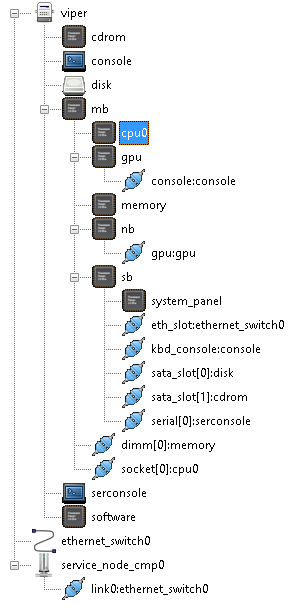
\includegraphics[width=0.6\textwidth]{x58-components}
    \caption{Конфигурация системы Viper}
    \label{fig:x58-components}
\end{figure}


\section{Устройства и классы Simics}

Базовая единица симуляции в Simics --- это объект. Объекты одного типа образуют класс. Классы в Simics имеют уникальные имена; встроенная справка по имени класса выдаёт всю информацию о свойствах объектов. Самые часто встречающие классы в Simics --- это \texttt{memory-space}, используемый для организации доступа к периферийным устройствам, размещённым в пространстве физической памяти, \texttt{ram} --- для моделирования ОЗУ и ПЗУ, и \texttt{image} --- для представления всех сущностей, хранящих группы адресуемых байт: ОЗУ, диски, кэши и т.п.

Самое важное назначение объектов Simics состоит в том, что большинство из них являются устройствами, эволюция которых во времени наблюдается при симуляции. Согласно принципам объектно-ориентированного программирования у них есть методы (группируемые в \textit{интерфейсы}) и поля (называемые в Simics \textit{атрибутами}).

\section{Компоненты}
Для удобства создания больших конфигураций виртуальных систем некоторые объекты, называемые \textit{компонентами}, выполняют лишь ограниченную связующую роль и практически не изменяются после того, как все участвующие в симуляции устройства соединены друг с другом. Задача компонент --- обеспечить на этапе создания конфигурации проверку правильности соединения устройств друг с другом. Например, очень часто используются две следующих компоненты: процессорный блок (\abbr package) и разъём на материнской плате для него (\abbr socket). Процессорный блок может содержать на себе несколько устройств-ядер процессора, каждое из которых надо соединить с ОЗУ и другими устройствами, находящимися в составе модели материнской платы. Модель разъёма на плате устроена так, что автоматически создаёт все необходимые соединения. В случае несовместимости компонент симулятор сообщает об ошибке, предотвращая ситуации, в которых конфигурация была создана лишь частично.

Отличие объектов-компонент от объектов-устройств состоит в том, что они очень редко модифицируются в ходе симуляции. Фактически они нужны только один раз, на этапе её создания. Их код необязательно должен быть быстрым --- достаточно обеспечить корректность. Поэтому практически всегда компоненты Simics пишутся на языке Python, процедуры которого, в отличие от языков, используемых для написания устройств --- Си, C++, DML, --- работают медленно. Однако скорость разработки компонент на Python ввиду его динамической природы значительно выше, а скорость финального кода практически не влияет на работу модели в целом.

\subsection{Иерархия устройств}

Корневой элемент создаваемой модели компьютера имеет имя, традиционно хранящееся сценариях конфигураций в переменной \texttt{\$system}. В нашем случае она содержит строку \texttt{"viper"}. Это имя используется для именования компонента шасси, на котором <<крепятся>> все остальные устройства. Это проявляется в том, что иерархические имена подкомпонент образованы присоединением к имени надкомпоненты своего имени через символ точки. Так, материнская плата данной системы имеет имя \texttt{viper.mb}, первый процессор на ней --- \texttt{viper.mb.cpu0}, а первое ядро в этом процессоре --- \texttt{viper.mb.cpu0.core[0][0]}. Следует отметить, что подобная иерархическая организация имён диктуется именно использованием механизма компонент; если устройства соединять <<вручную>>, то их имена могут и не образовывать иерархии.

Для просмотра списка всех устройств используйте команду \texttt{list-objects -recursive}. Альтернативно можно использовать окно \textbf{Object Browser} (рис.~\ref{fig:object-browser}).

\begin{figure}[htb]
    \centering
    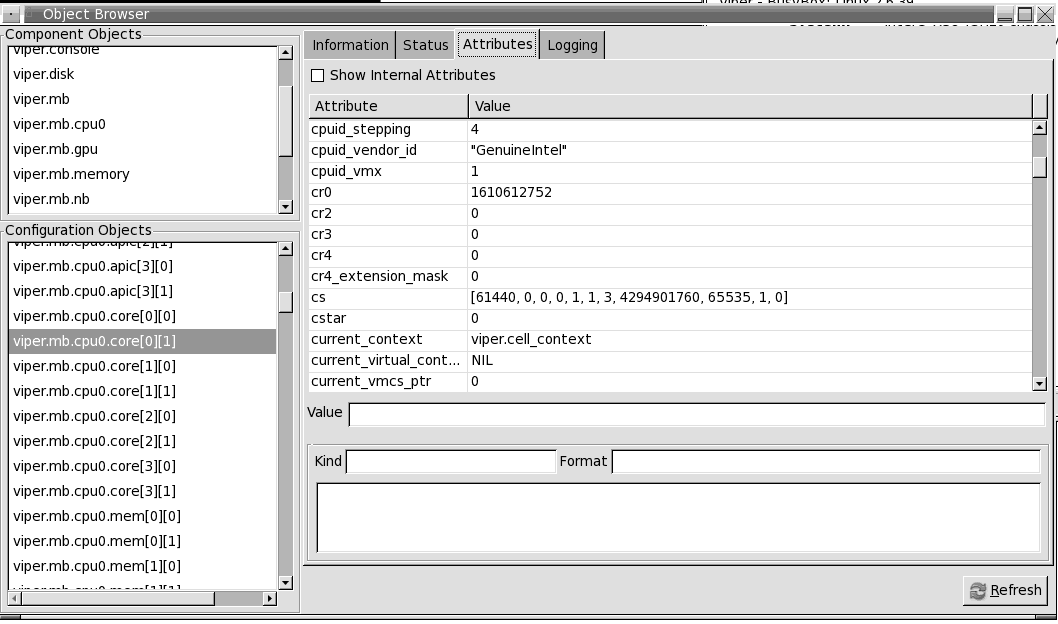
\includegraphics[width=0.8\textwidth]{win-object-browser}
    \caption{Окно для просмотра объектов и их атбрибутов}
    \label{fig:object-browser}
\end{figure}

\section{Команды}

Каждый класс моделей может предоставлять несколько команд, которые позволяют инспектировать или изменять состояние объектов данного класса. Самые часто реализуемые внутри классов команды --- это \texttt{status} и \texttt{info}. Для того, чтобы вызвать команду для некоторого устройства, следует указать её имя после имени устройства и символа <<точка>>.
Например, все устройства модели памяти имеют команды \texttt{get} и \texttt{set}, которые позволяют читать и записывать данные в симулируемую память:

\begin{lstlisting}
simics> viper.mb.cpu0.mem[0][0].get address = 0xffff0000
0x00
simics> viper.mb.cpu0.mem[0][0].set address = 0xffff0000 value = 0xaabbccdd
\end{lstlisting}

Аргументы любой команды можно узнать в справке к ней (команда \texttt{help <устройство>.<команда>}) или с помощью автодополнения (нажав клавишу \textbf{Tab}).

\subsection{Глобальные команды}

Кроме команд, специфичных для устройств, существуют так называемые глобальные команды, эффект которых состоит или в доступе к состоянию всей симуляции в целом, или же к текущему <<устройству>> некоторого класса, что позволяет сэкономить время на наборе иерархических имён. Например, команда \texttt{ptime} выводит значения симулируемого времени для текущего процессора, тогда как \texttt{ptime -all} позволяет увидеть аналогичную информацию о всех процессорах в системе.

\begin{lstlisting}
simics> ptime
processor                 steps   cycles   time[s]
viper.mb.cpu0.core[0][0]      0        0         0
\end{lstlisting}


\section{Диагностические сообщения}

Одно из назначений симуляторов --- помогать в разработке аппаратуры и программ для неё. При этом разработчикам необходимо понимать, какие события в каком порядке происходят во время симуляции и контролировать их корректность. Для этого все объекты Simics могут выводить диагностические сообщения в консоль управления Simics или в файл.


\subsection{Формат сообщений}
Пример сообщений при загрузке некоторой гостевой системы.

\begin{lstlisting}
simics>
[viper.mb.gpu.vga info] writing character   (0x20) at (30, 203) Attrib 0x7
[viper.mb.nb.core_scratch_gpio spec-viol] 4 byte read access at offset 0x100 in pci_config (addr 0xa1100) outside registers or misaligned access
[viper.mb.nb.core_control_status spec-viol] 4 byte read access at offset 0x100 in pci_config (addr 0xa2100) outside registers or misaligned access
[viper.mb.conf unimpl] QEMU_CFG_SMBIOS_ENTRIES unimplemented
[viper.mb.sb.ehci[1] spec-viol] Write to read-only field usb_regs.usbsts.hchalted (value written = 0, contents = 0x1).
\end{lstlisting}

В целом формат напоминает текст пьесы, в которой участвующие в ней персонажи по очереди произносят свои реплики.
Формат сообщения по умолчанию имеет вид \texttt{[device] type message}\footnote{С помощью команды \texttt{log-setup} в него можно добавить вывод значения виртуального времени на момент выдачи сообщения.}. Здесь
\begin{itemize}
    \item \texttt{device} --- имя устройства;
    \item \texttt{type} --- одна из следующих строк: <<info>> для информационных сообщений, <<unimpl>> для обозначения неполной точности в поведении модели, <<spec-viol>> для ситуаций, в которых моделируемое устройство вводится в режим, противоречащий спецификации модели, <<undef>> --- ситуации неопределённого поведения устройств, и <<error>> --- для обозначения ошибок в работе модели или симуляции в целом, после которых правильность работы не гарантируется;
    \item \texttt{message} --- собственно текст сообщения.
\end{itemize}

\subsection{Фильтрация диагностических сообщений}
Поскольку излишне частые и подробные сообщения могут засорить журнал, Simics предоставляет несколько механизмов для их фильтрации. С помощью команды \texttt{log-type} определяется, какие из типов сообщений будут выводиться, а какие будут игнорироваться. При этом можно установить фильтрацию как для отдельных объектов, так и для всей симуляции в целом.

Кроме того каждое сообщение, кроме типа error (они выводятся всегда), имеют уровень важности, выражаемый числом от 1 до 4. Сообщения уровня 1 самые важные, тогда как на четвёртом уровне обычно содержится информация, необходимая для отладки. При старте симуляции по умолчанию показываются только важные сообщения (первого уровня). Для управления тем, начиная с какого уровня они будут выводится, доступна команда \texttt{log-level}. Она может использована как глобальная, так и быть указанной для отдельных объектов:

\begin{lstlisting}
simics> log-level 4
New global log level: 4
simics> viper.mb.rom.log-level 3
[viper.mb.rom] Changing log level: 4 -> 3
\end{lstlisting}

\section{Атрибуты}

Атрибуты являются аналогом полей в объектах из парадигме ООП. В симуляции основная их задача состоит в хранении архитектурного состояния моделей. Обратиться к ним можно по их имени, указываемому после имени объекта, с помощью оператора стрелки <<\texttt{->}>>. Например, для просмотра содержимого регистров центрального процессора можно использовать соответствующие атрибуты:
\begin{lstlisting}
simics> viper.mb.cpu0.core[0][0]->rax
0
simics> viper.mb.cpu0.core[0][0]->rip
65520
simics> viper.mb.cpu0.core[0][0]->rdx
67233
simics> viper.mb.cpu0.core[0][0]->xmm
[[0, 0], [0, 0], [0, 0], [0, 0], [0, 0], [0, 0], [0, 0], [0, 0], [0, 0], [0, 0], [0, 0], [0, 0], [0, 0], [0, 0], [0, 0], [0, 0]]
\end{lstlisting}

Для изменения значения, хранимого в атрибуте, используется оператор присваивания <<\texttt{=}>>:
\begin{lstlisting}
simics> viper.mb.cpu0.core[0][0]->rax = 123
\end{lstlisting}

Естественно, что изменение атрибутов необходимо проводить очень аккуратно, так как их содержимое напрямую влияет на симуляцию. Например, если изменить значение атрибута \texttt{rip} и связанного с ним регистра \texttt{RIP}, то дальнейшее исполнение кода начнётся с нового места.

\subsection{Типы атрибутов}

По аналогии с переменными в языках программирования атрибуты имеют типы. При присвоении атрибуту нового значения с помощью присваивания производится проверка, что тип выражения с правой стороны соответствует его заявленному типу, и, если это не так, операция прерывается.

Типа каждого атрибута специфицируется при написании модели с помощью строки, символы которой определяют допустимые варианты входных значений.

\begin{enumerate*}
\item Скалярные. Имеют типы \texttt{"i"} (целое число), \texttt{"s"} (строка), \texttt{"b"} (булевый тип).
\item Объекты. Их тип --- \texttt{"o"}. С помощью таких атрибутов одни устройства могут вызывать методы других.
\item Списки. Они могут быть как однородными \texttt{"[iiii]"}, так и содержать элементы разных типов \texttt{"[oios]"}. Кроме того, их длина может быть переменной: \texttt{"[i*]"}.
\item Пустой тип \texttt{"n"}. В консоли он задаётся с помощью NIL или нуля.
\item Вариативный тип, значение которого может быть одним из нескольких ранее описанных: \texttt{"i|s|o"}.

\end{enumerate*}

Кроме того, некоторые атрибуты при регистрации могут быть помечены как псевдоатрибуты или атрибуты только для чтения. Почти всегда они не соответствуют <<настоящему>> архитектурному состоянию, а используются для более удобного представления информации об устройстве или для нужд отладки. Более подробно о них будет сказано в последующих главах.

\section{Задания}

\begin{enumerate*}
\item Найдите команду, перечисляющую все атрибуты заданного объекта. Перечислите все атрибуты объектов центральных процессоров \texttt{viper.mb.cpu0.core[0][0]}.
\item Найдите команду, перечисляющую все объекты текущей симуляции. Какие флаги она имеет и каково их назначение?
\item Изучите атрибуты и команды объекта \texttt{sim}. Какому устройству гостевой симуляции он соответствует?
\end{enumerate*}

\section{Контрольные вопросы}

\begin{enumerate*}
\item Перечислите известные вам способы получения справки по командам и моделям Simics.
\item Какие языки программирования чаще всего используются для написания моделей устройств Simics? Почему?
\item Чем, по-вашему, отличается объект с моделью устройства от объекта компонента?
\end{enumerate*}

\iftoggle{webpaper}{
    \printbibliography[title={Список литературы к занятию}]
}{}

% \section{Задания}
% 
%  В этой работе мы будем создавать небольшую симуляцию, состоящую из простой модели процессора класса \texttt{sample-risc} и модели оперативной памяти. Для этого необходимо будет создать и настроить индивидуальные объекты. Исходный скрипт находится в файле \texttt{script.py} (см. приложение~\ref{chap:app-broken-script}). Однако он содержит несколько ошибок, которые не позволяют это сделать сразу. Задание состоит в том, чтобы разобрать сообщения симулятора, внести модификации в исходный скрипт и запустить его.
% 
% Следующие замечания должны помочь в решении поставленной задачи.
% 
% \begin{itemize*}
%     \item Данный скрипт написан на языке Python и поэтому требует специального флага при указании его имени в командной строке.
%     \item Для выяснения списка опций используйте команду \texttt{simics -h}.
%     \item Переменные в Simics объявляются с помощь оператора <<\texttt{=}>>. Имена переменных начинаются со знака доллар, например \texttt{\$system}.
%     \item Перед выполнением второй фазы инициализации объектов все обязательные атрибуты предобъектов должны быть настроены.
%     \item Обращайте внимание на вывод сообщения об ошибках --- часто они содержат имя файла и номер строки.
%     \item Комментарии начинаются со знака <<диез>> \texttt{\#}.
% \end{itemize*}
